高低通滤波是数字图像处理领域的基础,
它可以混合图像的生成。
其核心原理在于理解图像的频率特性和卷积操作。

\subsection{图像频率}
图像可以被看作是二维信号,包含不同频率的信息。
低频成分对应于图像中变化缓慢的区域,如平滑的背景和大的结构轮廓。
高频成分对应于图像中变化快速的区域,如图像的边缘、纹理和细节。
通过分离和处理这些不同频率的成分,
我们可以实现图像的模糊、锐化或特征提取等操作。

\subsection{图像滤波与卷积}
图像滤波是通过卷积操作实现的。
卷积是将一个小的矩阵(称为滤波器或卷积核)与图像的局部区域进行加权求和的过程,如图1所示
\begin{figure}
	\centering
	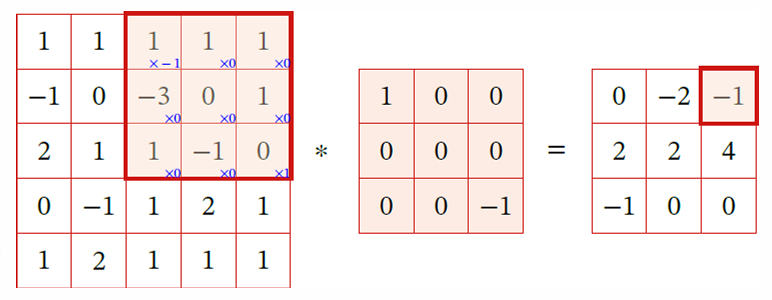
\includegraphics[width=0.7\linewidth]{image/convolution}
	\caption{卷积运算示意图}
	\label{fig:convolution}
\end{figure}


具体来说,滤波器在图像上滑动,在每个位置,将滤波器矩阵的元素与其覆盖的图像像素值相乘,
并将结果相加,得到输出图像在该位置的像素值。

\subsection{滤波器}
低通滤波通过卷积一个低通滤波器(如高斯滤波器)实现,
它可以平滑图像,去除高频噪声和细节,保留图像的整体结构和颜色。
高通滤波的一种常用实现方式是:从原始图像中减去其低通滤波后的结果。
低通滤波保留了图像的低频信息,去除高频信息。
当用原始图像减去低频图像时,剩余的部分就是原始图像中的高频信息。
这允许我们提取或增强图像的边缘和细节。

\subsection{混合图像的生成}
混合图像(Hybrid Image)是结合了两张不同图像的频率成分而创建的。
其原理基于人类视觉系统的特性:在近距离观察时,
人眼更容易感知图像的高频细节;
在远距离观察时,则更容易感知图像的低频轮廓。
通过将一张图像的低频成分与另一张图像的高频成分叠加合成,
我们可以创建出一种在不同观察距离下呈现不同内容的图像。具体实现步骤如下:
\begin{enumerate}
    \item 对第一张图像进行低通滤波,提取其低频成分。
    \item 对第二张图像进行高通滤波,提取其高频成分(通过原始图像减去低通滤波结果)。
    \item 将第一张图像的低频成分与第二张图像的高频成分相加,生成混合图像。
    \item 对生成的混合图像像素值进行裁剪,确保其在有效的显示范围内。
\end{enumerate}

通过调整低通滤波器(高斯滤波器)的截止频率,我们可以控制保留多少低频信息和高频信息,从而影响混合图像在不同距离下的视觉效果。
